\documentclass[mathserif, aspectratio=169]{beamer}

\usepackage{psfrag,graphicx}
\usepackage{amsmath}
\usepackage[absolute,overlay]{textpos}

\usepackage{braket}
\graphicspath{{figs/}}

\usetheme{Boadilla}
\makeatother
\setbeamertemplate{footline}[frame number]

\usepackage{graphicx}
\usepackage{caption}
\usepackage{subcaption}
\captionsetup{compatibility=false}
\usepackage{amsmath} 
\usepackage{amssymb} 
\usepackage{amsthm}  
\usepackage{bm}
\usepackage{lipsum}
\usepackage[linesnumbered, ruled]{algorithm2e}
\usepackage{color}
\newtheorem{assumption}{Assumptions}
\newtheorem{prop}{Proposition}
\newtheorem{defn}{Definition}
\newtheorem{thm}{Theorem}
\newtheorem{lem}{Lemma}
\newtheorem{cor}{Corollary}
\newtheorem{sol}{Decentralized Solution}
\newtheorem{thresh}{$\epsilon$-thresholding}
\definecolor{light-gray}{gray}{0.8}
\usepackage{textcomp}

\newcommand{\backupbegin}{
   \newcounter{finalframe}
   \setcounter{finalframe}{\value{framenumber}}
}
\newcommand{\backupend}{
   \setcounter{framenumber}{\value{finalframe}}
}
\newcommand{\norm}[1]{\left\lVert #1 \right\rVert}

\makeatletter
\setbeamertemplate{navigation symbols}{}

\title[Lecture 20] % (optional, use only with long paper titles)
{Data, Environment and Society: \\{Lecture 20: Support Vector Machines}}



\author[ER131: Data, Environment and Society] 
{Instructor: Duncan Callaway\\
GSI: Salma Elmallah} 

%\logo{
%\includegraphics[width=1.5cm,height=1.5cm,keepaspectratio]{uvic_logo_h.jpg}
%}
\vspace{-20mm}
\institute[UC Berkeley] % (optional, but mostly needed)
 {\small{ \bf November 7, 2019}}


\date[November 7, 2019]



\begin{document}

\frame{
  \titlepage
}

\begin{frame}{}
\includegraphics[height=\textheight]{new_yorker}
\end{frame}

\begin{frame}{Announcements}

\begin{itemize}
\item I'll be teaching from ISLR Ch 9 today.
\item HW9 due today!
\item Next week lab: come with data and resource allocation question in hand.
\item Thursday: Guest lectures from Diego Ponce de Leon and Grace Wu -- come ready to ask questions!
\end{itemize}

\end{frame}

\begin{frame}{Objectives for today}
\begin{itemize}
\item Some examples
\item Introduce the idea of a \textbf{hyperplane} (it's really simple)
\item Figure out what a \textbf{maximal margin hyperplane} (MMH) is and why we use it
\begin{itemize}
\item Note, these only work for \textit{separable data}
\end{itemize}
\item Understand how \textbf{support vector classifiers} extend the MMH to cases when the data are not separable.  
\begin{itemize}
\item SVCs are \textit{linear} separations of the feature space
\end{itemize}
\item Open your horizons to the \textbf{support vector machine}
\begin{itemize}
\item This provides nonlinear separations of the feature space!
\end{itemize}
\end{itemize}

\end{frame}

\begin{frame}{Motivating examples: Society}

face recognition

\includegraphics[scale=0.25]{murray_hackernoon_2017_face}
 %https://hackernoon.com/building-a-facial-recognition-pipeline-with-deep-learning-in-tensorflow-66e7645015b8

character recognition, 

\includegraphics[scale=0.45]{thome_character}% http://cdn.intechopen.com/pdfs/40722/InTech-Svm_classifiers_concepts_and_applications_to_character_recognition.pdf
\hspace{20mm}\includegraphics[scale=0.18]{malik_2009_handwriting}
%https://www2.eecs.berkeley.edu/Pubs/TechRpts/2009/EECS-2009-159.html

\end{frame}

\begin{frame}{Motivating examples -- environment}

\includegraphics[scale=0.6]{lu_etal_OzoneSVM}

%\includegraphics[scale=0.2]{Shi_etal_ForecastingPower}

\i%ncludegraphics[scale=0.2]{depuru_etal_SVMTheft}

%electricity theft %http://ieeexplore.ieee.org/document/5772466/

%solar production % https://ieeexplore.ieee.org/abstract/document/6168891

%ozone prediction %https://www.sciencedirect.com/science/article/pii/S0048969708000776


\end{frame}


\begin{frame}{Motivating examples -- environment}

%\includegraphics[scale=0.3]{lu_etal_OzoneSVM}

\includegraphics[scale=0.4]{Shi_etal_ForecastingPower}

%\includegraphics[scale=0.2]{depuru_etal_SVMTheft}

%electricity theft %http://ieeexplore.ieee.org/document/5772466/

%solar production % https://ieeexplore.ieee.org/abstract/document/6168891

%ozone prediction %https://www.sciencedirect.com/science/article/pii/S0048969708000776

\end{frame}


\begin{frame}{Motivating examples -- environment}

%\includegraphics[scale=0.3]{lu_etal_OzoneSVM}

%\includegraphics[scale=0.2]{Shi_etal_ForecastingPower}

\includegraphics[scale=0.4]{depuru_etal_SVMTheft}

%electricity theft %http://ieeexplore.ieee.org/document/5772466/

%solar production % https://ieeexplore.ieee.org/abstract/document/6168891

%ozone prediction %https://www.sciencedirect.com/science/article/pii/S0048969708000776


\end{frame}


\begin{frame}{The hyperplane}
\begin{columns}
\column{0.4\textwidth}
\begin{itemize}
\item A point splits a 1-dimensional space in two
\vspace{5mm}
\item A line splits a 2-dimensional space in two
\vspace{5mm}
\item A plane splits a 3-dimensional space in two
\vspace{5mm}
\item A hyperplane splits a $p$-dimensional space in two.  
\end{itemize}
\column{0.6\textwidth}

\end{columns}
\end{frame}

\begin{frame}{Mathematical representation}

If we have a line defined by

\begin{align*}
x_2 = -2+\frac{1}{2} x_1
\end{align*}

Then the equality defining the hyperplane is:

\vspace{15mm}
or

\vspace{15mm}
\end{frame}

\begin{frame}{How we'll think about the hyperplane}

\begin{itemize}
\item In a data set with $p$ features...
\item We'll conceive of it as a $p-1$ dimensional object 
\item ...and we'll identify the location of observations in relation to the hyperplane
\end{itemize}

\vspace{10mm}
\begin{columns}
\column{0.5\textwidth}

\column{0.5\textwidth}
On the hyperplane:
\vspace{10mm}

Above the hyperplane:
\vspace{10mm}

Below the hyperplane:
\end{columns}
\end{frame}

\begin{frame}{Theoretical example: Classification with hyperplanes}
\begin{columns}
\column{0.5\textwidth}
Suppose we have
\begin{itemize}
\item \textcolor{blue}{blue points}
\item \textcolor{red}{red points}
\end{itemize}
\vspace{10mm}
A ``separating hyperplane'' has the property that:

\column{0.5\textwidth}

\end{columns}

\end{frame}

\begin{frame}{Using the plane for predictions}
\begin{columns}
\column{0.5\textwidth}
This part is simple.  If we have a test observation, we simply evaluate $f(x_\text{test})$ and assign it to a class on the basis of the sign of the result.
\column{0.5\textwidth}

\end{columns}
\end{frame}

\begin{frame}{How to choose the location of the plane?}
\begin{columns}
\column{0.5\textwidth}
Let's pose this as a learning problem.  We have data and we'd like to place the hyperplane in between the two classes.

\begin{itemize}
\item First: What does  large $|f(x_i)|$ imply?  \uncover<2->{$\rightarrow$ A point is far from the hyperplane.}
\end{itemize}
\vspace{5mm}
\uncover<3->{Now, how should we choose which plane to draw?
\vspace{5mm}

The rest of this lecture focuses on how to draw these separating geometries}

\column{0.5\textwidth}

\end{columns}
\end{frame}

\begin{frame}{Maximal margin hyperplane (MMH)}

\begin{columns}
\column{0.5\textwidth}
\begin{itemize}
\item MMH defined: The MMH is the hyperplane that \textit{maximizes} the \textit{smallest distance} between the plane and all data.
\begin{itemize}
\item In other words: it is the plane that is farthest from the data.
\end{itemize}
\item Important: This requires that the data are \textit{linearly separable.  }
\end{itemize}
\column{0.5\textwidth}

\end{columns}
\end{frame}

\begin{frame}{How many points define the hyperplane?}

\begin{columns}
\column{0.5\textwidth}
In two dimensions...
\begin{itemize}
\item What is the smallest number of points that could define the hyperplane?
\vspace{5mm}
\item What is the largest number of points that could define the hyperplane?
\vspace{5mm}
\end{itemize}
...We call these points ``support vectors'' because each of the 2-3 observations is a ``vector'' of information that supports the plane.

\end{columns}

\end{frame}

\begin{frame}{Variance alert}

In two dimensions, three observations determine the parameters of the model.  Or more generally $p+1$ parameters.  \textit{If} $p$ is small, this leads to high variance across training data sets.   
\end{frame}

\begin{frame}{And now for the math}

We'll solve for the location of the MMH using...\pause you guessed it, optimization.  

\vspace{40mm}

\end{frame}

\begin{frame}{Pause for a moment...}
The location of the MMH is very sensitive to the support vectors:

\includegraphics[width=0.7\textwidth]{ISLR_9point5}

Furthermore:
\begin{itemize}
\item Though the $M$ objective in the MMH formulation \textit{can} in principle be negative (which allows for non-separable data)...
\item ...the problems of variance get worse as data become non-separable.
\end{itemize}
\end{frame}

\begin{frame}{Support vector \textit{classifiers}}
\begin{columns}
\column{0.5\textwidth}
Can we get
\begin{itemize}
\item ...less sensitivity to individual observations, and
\item ...better classification for most training data (at expense of some poor classifications)
\end{itemize}
The answer is yes -- but we will
\begin{itemize}
\item Allow some training data to enter the ``margin''
\item ...and perhaps even be on the wrong side of the hyperplane.
\end{itemize}
Now we call the margin a ``soft margin''
\column{0.5\textwidth}

\end{columns}
\end{frame}

\begin{frame}{Support vector classifier details}

\begin{columns}
\column{0.5\textwidth}
We'll solve a slightly different optimization problem.
\begin{itemize}
\item Still classifies observations on the basis of what side of the hyperplane they're on
\item But a few observations can be mis-classified.
\end{itemize}
\column{0.5\textwidth}
The optimization problem is: 
\vspace{40mm}
\end{columns}
\end{frame}

\begin{frame}{What are the $\epsilon_i$?}

\begin{columns}
\column{0.5\textwidth}
\begin{itemize}
\item Each \textit{observation} gets its own $\epsilon_i$.  
\item The $\epsilon$ are decision variables -- the optimization problem will solve for them.  
\item Without $C$, we'd just give everyone an $\epsilon$ and go on a misclassification binge.  
\item But with $C$, the $\epsilon$ values are chosen within a budget. 
\begin{itemize}
\item $\epsilon_i = 0$, no margin violation
\item $0<\epsilon_i<1$, in the margin but on the correct side of the plane
\item  $\epsilon_i>1$, on the wrong side of the plane.  
\end{itemize}
\end{itemize}
\column{0.5\textwidth}
\end{columns}
\end{frame}

\begin{frame}{Tuning $C$}
\begin{columns}
\column{0.6\textwidth}
\includegraphics[height = 0.9\textheight]{small_vs_big_C}
\column{0.4\textwidth}
Questions
\begin{enumerate}
\item Which plot has large $C$?  Which is small?
\item What's going to have the highest variance?  Large or small $C$?
\end{enumerate}

\end{columns}
\end{frame}

\begin{frame}{But decision boundaries aren't always so simple...}

\begin{columns}
\column{0.5\textwidth}
What if the boundary looked like this?
\vspace{40mm}
\column{0.5\textwidth}
We might get better performance if we replaced the constraint in the optimization problem:

\vspace{40mm}

\end{columns}
\end{frame}


\begin{frame}{Setup for SVM ``Kernels'': Linear boundary}



\begin{columns}
\column{0.5\textwidth}
\vspace{10mm}

Let $\braket{x_i,x_k} = \sum_{j=1}^px_{ij}x_{kj}$

\vspace{5mm}

One can show that:

%\vspace{5mm}
\begin{align*}
\beta_0 + \sum_{j=1}^p \beta_j x_{ij} &\Leftrightarrow \beta_0 + \sum_{k=1}^n \alpha_k \braket{x_i,x_k}
\end{align*}

\column{0.5\textwidth}
\vspace{50mm}
What's the relationship between $\alpha$ and $\beta$?
\end{columns}
\end{frame}


\begin{frame}{SVM Kernels}
\begin{columns}
\column{0.7\textwidth}

\begin{align*}
K_\text{linear}(x_i,x_k) &= \braket{x_i,x_k} = \sum_{j=1}^px_{ij}x_{kj}\\
K_\text{polynomial}(x_i,x_k) &= (1+ \sum_{j=1}^px_{ij}x_{kj})^d\\
K_\text{radial}(x_i,x_k) &= \exp(-\gamma \sum_{j=1}^p(x_{ij}-x_{kj})^2)\\
\end{align*}

Then we can apply these kernels:
\begin{align*}
f(x_i) = \beta_0+\sum_{k=1}^p \alpha_k K(x_i,x_k) 
\end{align*}
\column{0.3\textwidth}

The radial kernel serves to give training observations far from a test point less weight (due to negative exponential). 

\vspace{5mm}

For the radial kernel, all the data comprise the model -- analogous to KNN.  
\end{columns}

\end{frame}

\begin{frame}{What do the kernels look like?}
\begin{columns}
\column{0.7\textwidth}

\includegraphics[scale=0.8]{SVM_kernels}

\column{0.3\textwidth}

Left: Polynomial, $d=3$.  Right: Radial.

\vspace{5mm}
Note that $d$ and $\gamma$ are parameters to tune (via cross validation!)
\end{columns}
\end{frame}

\begin{frame}{SVM Example}

\begin{figure}
\includegraphics[width=\textwidth]{shao_JPRS}
\caption*{}
\end{figure}
\end{frame}


\begin{frame}{Shao and Lunetta setup}
Loads of remote sensing data (MODIS):
\begin{itemize}
\item 46 input features for each 250 m$^2$ pixel
\begin{itemize}
\item 23 short wave infrared (SWIR) surface reflectance
\item 23 Enhanced Vegetation Index metrics -- basically a summary of the wavelengths
\end{itemize}
\item Training data from National Land Cover Dataset (NLCD), classifying land as
\begin{itemize}
\item urban, 
\item deciduous forest, 
\item evergreen forest, 
\item agricultural land, and 
\item wetland
\end{itemize}

\item Question: How do SVM, Neural networks (coming soon!), and regression trees perform relative to one another?
\end{itemize}
\end{frame}


\begin{frame}{Shao and Lunetta SVM Result}

\begin{figure}
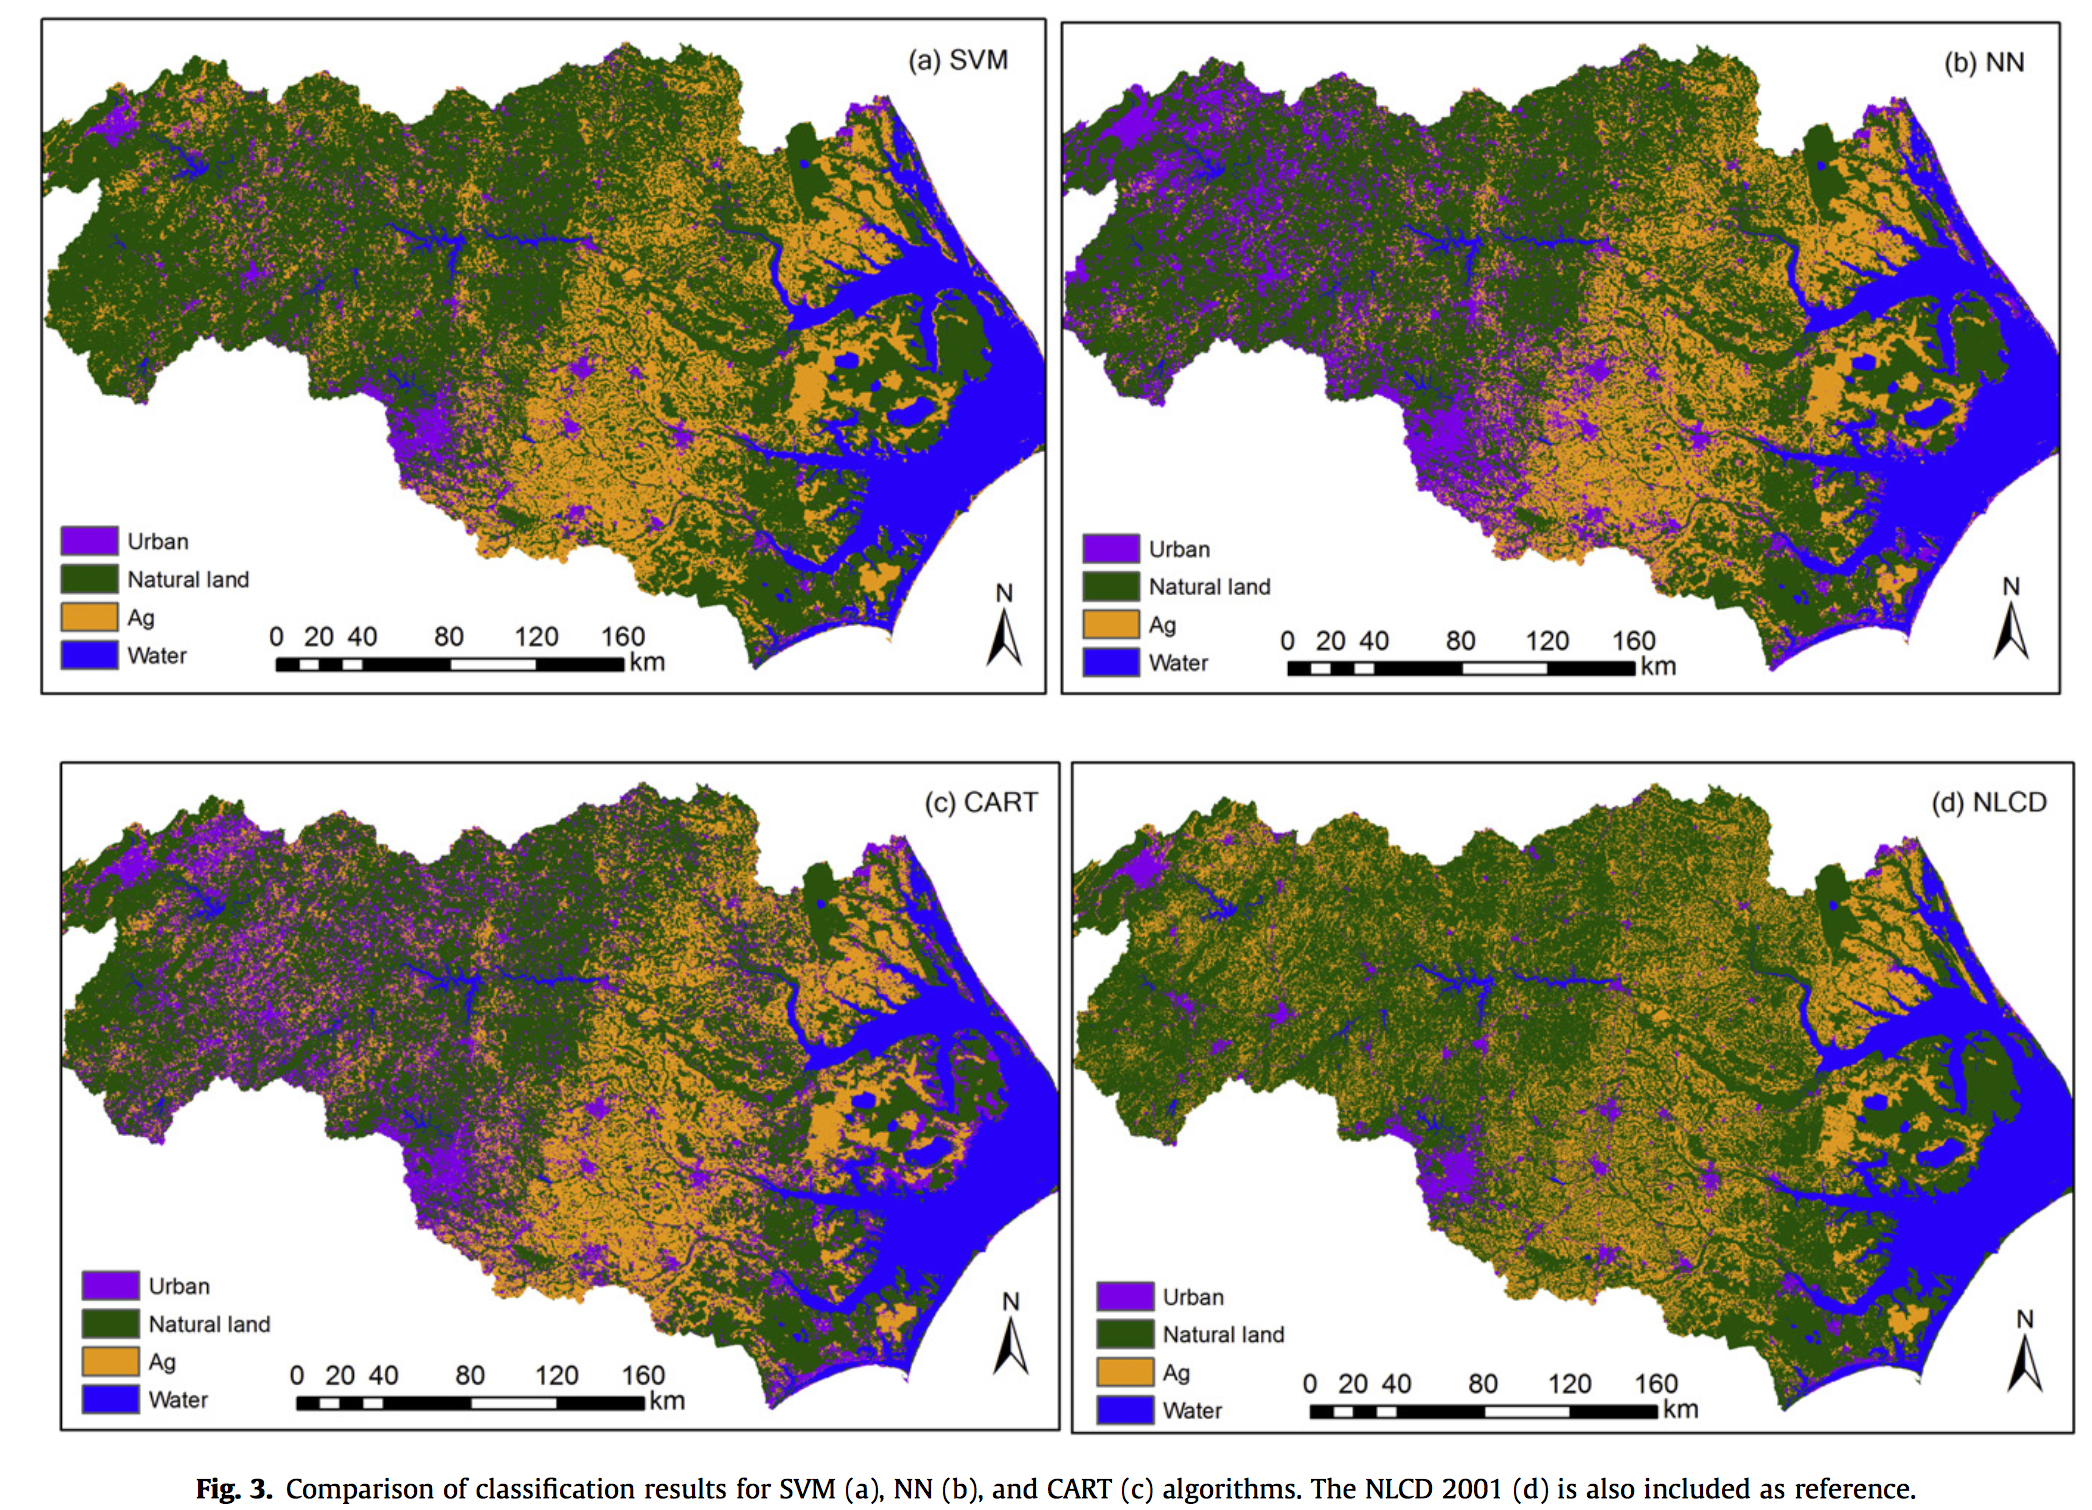
\includegraphics[height=0.9\textheight]{shao_figure}
\caption*{}
\end{figure}
\end{frame}

\begin{frame}{}
\begin{figure}
\includegraphics[height=\textheight]{shao_performance}
\caption*{}
\end{figure}
\end{frame}

\begin{frame}{Textbook example: Heart Data}
First: Receiver operating characteristic (ROC)\\~\\

\textbf{Sensitivity} = the fraction of ``positives'' that are correctly identified as positives  \\~\\

\textbf{Specificity} = fraction of negatives that we correctly identify as negatives \\~\\

\textbf{True positive rate} = sensitivity\\~\\

\textbf{False positive rate} = $1-$ specificity

Ideal classifiers have large true positive rate and low false positive.  \\~\\

For a given method, there are usually parameters one can tune to explore the tradeoff between true and false positives.  
\end{frame}

\begin{frame}{Classifying heart disease}
\begin{figure}
\includegraphics[width=\textwidth]{fig9_10}
\caption*{}
\end{figure}
\end{frame}

\begin{frame}{Classifying heart disease -- test data}
\begin{figure}
\includegraphics[width=\textwidth]{fig9_11}
\caption*{}
\end{figure}
\end{frame}

\begin{frame}{Interpreting Heart data result}
SVC is better than LDA, though surprisingly not by much if one recalls how simple the LDA approach is.\\~\\

On training data, SVM with radial kernels are exceptional \\~\\

...But not so much on test data.  Why?\\~\\
\pause

The decision boundary is really ``wiggly'' and prone to overfit. \\~\\

It appears that SVC would have lower variance / higher bias and they balance perfectly in  this particular case.

\end{frame}

\begin{frame}{Speaking of wiggly boundaries: From Elements of Statistical Learning}

\begin{figure}
\includegraphics[width=0.415\textwidth]{ESL_12_2a}\includegraphics[width=0.4\textwidth]{ESL_12_2b}
\caption*{These boundaries constructed with SVC.  Purple is ``truth'' (what they used to generate the data).  Note!  In ESL $C$ is the inverse of $C$ in ISLR.  So large $C$ here corresponds to small $C$ there, and vice versa.}
\end{figure}

\end{frame}

\begin{frame}{One more example: From Elements of Statistical Learning}

\begin{figure}
\includegraphics[width=0.4075\textwidth]{ESL_12_3a}\includegraphics[width=0.4\textwidth]{ESL_12_3b}
\caption*{These boundaries constructed with SVM. Purple is ``truth'' (what they used to generate the data).  }
\end{figure}

\end{frame}

\end{document}
